
\section{Toric Construction of Models}

In this section we discuss the results of \cite{tim} which gives a method of explicitly constructing a regular normal crossings model of a curve and explicitly describing its special fiber using the preceding methods characterizing curves on toric surfaces. 
\begin{rmk}
In \cite{tim}, Dokchitser often uses ``curve'' to refer to an integral separated \textit{geometrically connected} scheme of finite type over a field. To mitigate any confusion, we render any results quoted from his work with ``curve'' replaced by ``geometrically connected curve'' when necessary.
\end{rmk}

\subsection{Notations and Definitions}

We work in the case of a discretely definition valued field $K$ with valuation $\nu : K^\times \onto \Z$, valuation ring $R$, uniformizer $\varpi$, and residue field $\kappa$. Given a smooth projective geometrically connected curve over $K$ our goal will be to construct a regular normal crossings model over $R$. First we need to fix some notation.

\begin{defn}
Given a Laurent polynomial $f \in K[x^{\pm 1}, y^{\pm 1}]$ recall the Newton polygon is,
\[ \Delta(f) = \Conv{ \{ (i,j) \in \Z^2 \mid a_{ij} \neq 0 \} } \subset \R^2 \]
We will assume throughout that $\vol{\Delta} > 0$. 
Now we refine the Newton polygon with respect to the valuation $\nu : K^\times \onto \Z$,
\[ \Delta_\nu(f) = \mathrm{LowerConvHull} \left( \{ (i, j, v(a_{ij})) \mid (i, j) \in \Delta(f) \cap \Z^2 \} \right) \subset \R^2 \times \R \]
The projection $\pi : \Delta_\nu \to \Delta$ is a homomorphism. Thus,
for each point $P \in \Delta$ there is a unique point $(P, \nu(P)) \in \Delta_\nu$ which defines a piece-wise affine function $v : \Delta \to \R$ extending the valuation. 
\bigskip\\
The bijection $\pi : \Delta_\nu \to \Delta$ pushes the polyhedral structure on $\Delta_\nu$ onto $\Delta$. Because $\Delta_\nu$ is the lower convex hull of finitely many points in $\R^2 \times \R$ it decomposes into faces of dimension $0, 1, 2$. Under the projection $\pi : \Delta_\nu \to \Delta$ the $v$-\textit{vertices} $P$ of $\Delta$ are the images of the $0$-faces, the $v$-\textit{edges} $L$ are the images of the $1$-faces, the $v$-\textit{faces} $F$ are the images of the $2$-faces. These define a polygonal partition of $\Delta$. 
\end{defn}

\begin{defn}
For each edge $L$ and face $F$ there is an associated integer $\delta_\lambda$ (with $\lambda = L$ or $F$), the \textit{denominator}, defined as smallest positive $m$ such that $\nu(P) \in \frac{1}{m} \Z$ for each $P \in \lambda \cap \Z^2$. 
\end{defn}

\begin{rmk}
We now consider how to restrict a polynomial with respect to the $\nu$-partition to form a Laurent polynomial supported on the faces and vertices. First, following the Notation of \cite{tim} we define how to restrict the polynomial to some subset of a lattice.
\end{rmk}

\begin{defn}[Restriction]
Let $S \subset \Z^n$ be a nonempty subset of a lattice and take $\Lambda$ to be the smallest affine lattice $S \subset \Lambda \subset \Z^n$ containing $S$. Let $\Lambda$ have rank $r$ and choose an isomorphism $\phi : \Z^r \to \Lambda$. Then for a Laurent polynomial $g \in K[\bf{x}^{\pm 1}]$ we define the restriction $g|_S \in K[\bf{y}^{\pm 1}]$,
\[ g|_S = \sum_{\bf{i} \in \phi^{-1}(S)} c_{\phi(\bf{i})} \bf{y}^{\bf{i}} \in K[\bf{y}^{\pm 1}] \quad \text{for} \quad g = \sum_{\bf{i} \in \Z^n} c_{\bf{i}} \bf{x}^{\bf{i}} \]
Note that different choices of an isomorphism $\Lambda \to \Z^r$ are related by an automorphism in $\GL{r}{\Z}$ acting on the variables $\bf{y}$. 
\end{defn}

\begin{rmk}
The notational complexity of the above definition derives from making the polynomial $g|_S$ an element of a standard Laurent polynomial ring $k[\bf{y}^{\pm 1}]$. We can simplify the above notation using our previous abstract notation used for the toric constructions. Given a lattice $M$ and a Laurent polynomial $g \in K[M]$ and a subset $S \subset M$ we define the restriction,
\[ g|_S = \sum_{m \in S} c_m \chi^m \in K[\left< S \right>] \quad \text{where} \quad g = \sum_{m \in M} c_m \chi^m \]
where $\left< S \right>$ is the sublattice of $M$ generated by $S$. The above definition is recovered choosing some isomorphism $\phi : \left< S \right> \to \Z^r$ giving an isomorphism $K[\left< S \right>] \cong K[\bf{y}]$. 
\end{rmk}

\begin{defn}[Reduction]
For a Laurent polynomial $h \in K[x^{\pm 1}, y^{\pm 1}]$, there exist integers, $c, m, n \in \Z$ such that $\tilde{h}(x, y) = \varpi^c h(\varpi^m x, \varpi^n y)$ has coefficients in $R$ and $\tilde{h} \mod \varpi \in \kappa[x, y]$ has the same Newton polygon as $h$. Then we say that $\overline{h} = \tilde{h} \mod \varpi$ is \textit{reduction} of $h$. 
\end{defn}

\begin{defn}
In particular for $\lambda$ an edge $L$ or face $F$ we define the restriction $f |_\lambda = f|_S$ for the set, $S = \{ P \in \lambda \cap \Z^2 \mid \nu(P) \in \Z \}$. Note, $S$ contains the vertices of $L$ or $F$.  
\end{defn}

\begin{rmk}
Reduction gives, for each edge $L$ and face $F$, polynomials $\overline{f|_L} \in \kappa[t]$ and $\overline{f|_F} \in \kappa[x, y]$. This gives affine curves over $\kappa$ on each edge and face which we complete in a toric compactification as follows.
\end{rmk}

\begin{defn}[Components]
We define the following schemes over $\kappa$:
\begin{enumerate}
\item $X_L = V(\overline{f_L}) \subset \Gm{\kappa}$ 
\item $X_F = V(\overline{f_F}) \subset \Gm{\kappa}^2$
\item $\overline{X}_F = X_F^\Delta$ is the completion of $X_F$ with respect to its Newton polygon $F$ i.e. the closure of the immersion $X_F \embed \Gm{\kappa}^2 \embed \Toric_F$. By Theorem \ref{baker_refinement}, $\overline{X}_F$ is connected and, in fact, the Theorem applies for any finite extension $\kappa' \supset \kappa$ showing that $\overline{X}_F$ is geometrically connected.
\end{enumerate}
\end{defn}

\begin{defn}
We say that $f \in k[x^{\pm 1}, y^{\pm 1}]$ is \textit{strictly} $\Delta_\nu$-\textit{regular} if all $X_F$ and $X_L$ are smooth over $\kappa$. 
\end{defn}

\begin{rmk}
The condition that all $X_L$ are smooth implies that $f$ is nondegenerate with respect to its Newton polygon since it implies that $f$ restricted to each edge is smooth. 
\end{rmk}

\begin{defn}
A Laurent polynomial $f \in K[x^{\pm 1}, y^{\pm 1}]$ is $\Delta_\nu$-\textit{regular} if each $X_F$ is smooth and for the interior edges $L$ and edges $L \subset \partial F$ with $\delta_L \neq \delta_F$ we require $X_L$ is smooth and otherwise we require $\overline{X}_F$ is \textit{outer-regular} i.e. smooth at the points corresponding to $L$ via the bijection of $\Gal{\kappa^\sep / \kappa}$-sets,
\[ \overline{X}_F(\bar{\kappa}) \setminus X_K(\bar{\kappa}) \longleftrightarrow \coprod_{L \supset \partial F} X_L(\bar{\kappa}) \]
which derives from Baker's theorem. Since $\overline{X}_F$ is a toric compactification of $X_F$, the additional points correspond to the vanishing of the equation along the toric divisors which correspond to edges $L \subset \partial F$ so smoothness of $\overline{X}_F$ is ensured by outer-regularity.
\end{defn}

\begin{rmk}
As with toric regularity, we have defined the notion of $\Delta_\nu$-regular with respect to a given Laurent polynomial i.e. to a given affine model $C_0$ of a curve. As before, we extend this definition to an arbitrary curve in the obvious way.
\end{rmk}

\begin{defn}
A curve $C$ over $K$ is (strictly) $\Delta_\nu$-regular if $C$ is birationally equivalent to some affine $U_f \subset \Gm{K}^2$ for some (strictly) $\Delta_\nu$-regular Laurent polynomial $f \in K[x^{\pm 1}, y^{\pm 1}]$. 
\end{defn}

\begin{rmk}
We need one more notion in order to describe the model of $C$ which is a combinatorial connectivity between two adjacent faces $F_1, F_2$ sharing an edge $L$. 
\end{rmk}

\begin{defn}[Slopes]
Edges are either \textit{inner/interior} meaning they form the boundary between two $\nu$-faces $F_1$ and $F_2$ or \textit{outer/exterior} on the boundary of $\Delta$. For an edge $L$ there is a unique affine function $L^*_{(F_1)} : \Z^2 \onto \Z$ with $L^*_{(F_1)} |_L = 0$ and $L^*_{(F_1)}|_{F_1} \ge 0$. Then the edge has two corresponding integers called the \textit{slopes} Defined as follows. Choose $P_0, P_1 \in \Z^2$ with $L^*_{(F_1)}(P_0) = 0$ and $L_{(F_1)}^*(P_1) =1$. Then,
\[ s_1^L = \delta_L (\nu_1(P_1) - \nu_1(P_0)) \quad \quad s_2^L = 
\begin{cases}
\delta_L (\nu_2(P_1) - \nu_2(P_0)) & L \text{ inner}
\\
\lfloor s_1^L - 1 \rfloor & L \text{ outer}
\end{cases} \]
where $\nu_i : \Z^2 \onto \Z$ is the unique affine function which agrees with $\nu$ on $F_i$ (recall that the faces are defined such that $\nu$ is affine when restricted to each face. Given the slopes, we may consider a sequence of rational numbers $\frac{m_i}{d_i} \in \Q$ such that,
\[ s_1^L = \frac{m_0}{d_0} > \frac{m_1}{d_1} > \frac{m_2}{d_2} > \cdots > \frac{m_r}{d_r} > \frac{m_{r+1}}{d_{r+1}} \quad \text{and} \quad 
\begin{vmatrix}
m_i & m_{i+1}
\\
d_i & d_{i+1}
\end{vmatrix} = m_i d_{i+1} - m_{i+1} d_i = 1 \]
Then $r(L)$, the minimal length of this sequence, and the denominators $d_i$ of this minimal sequence, are important combinatorial parameter of the edge $L$. It turns out such a minimal sequence is unique.
\end{defn}

\begin{rmk}
The existence of such a sequence needs some consideration. Take all rational numbers in $[s_1^L, s_2^L] \cap \Q$ with denominators bounded by the largest denominator of $s_1^L$ and $s_2^L$. This is a shifted Farey series. We define the Farey series $F^n$ to be the ordered sequence of rational numbers with denominator less than or equal to $n$ put in lowest terms. Then, if $\frac{a}{b} < \frac{c}{d}$ are consecutive terms in the Farey series then $\frac{c}{d} - \frac{a}{b} = \frac{1}{bd}$. Therefore,
\[ \begin{vmatrix}
a & c 
\\
b & d 
\end{vmatrix}
= ad - bc = 1 \] 
\cite[Remark 3.15]{tim} and \cite[Ch. III, Thm. 28, Thm. 29]{HW}.
Furthermore, if the sequence in $[s_1^L, s_2^L] \cap \Q$ with bounded denominators contains consecutive terms,
\[ \frac{a}{b} > \frac{a + c}{b + d} > \frac{b}{d} \]
then we must have,
\[ a(b + d) - b(a + c) = ab + ad - ab - bc = ad - bc = 1 \]
meaning that $\frac{a}{b} > \frac{b}{d}$ have the required adjacency property and thus $\frac{a + c}{b + d}$ may be removed from the sequence. We will be able reinterpret this as a blow-down of regular normal crossings models after we state the main theorems describing the structure of such models from the above combinatorial data.
\end{rmk}

\subsection{Main Theorems}

We describe the properties of a model $\C_\Delta$ over $R$ associated to some polygonal partition of $\Delta$ defined by the Laurent polynomial $f \in K[x^{\pm 1}, y^{\pm 1}]$. The construction of $\C_\Delta$ proceed by defining a two-dimensional fan $\Sigma$ in $\R^3$ determined by the numerical parameters of $\Delta_\nu$ and to glue affine schemes $X_\sigma = \Spec{R[\sigma^\vee \cap \Z^3]}$ to produce a toric-like scheme $X_\Sigma$ over $\Spec{R}$. The generic fiber of $X_\Sigma \to \Spec{R}$ is a toric surface over $K$ thus containing $\Gm{K}^2 \embed (X_\Sigma)_K \embed X_\Sigma$ where the generic fiber is open in $X_\Sigma$ because $\Spec{K}$ is open in $\Spec{R}$. Then $\C_\Delta \subset X_\Sigma$ is the closure of $V(f) \subset \Gm{K}^2 \embed \Gm{R}^2 \embed X_\Sigma$. See \cite[Section 4]{tim} for details.

\begin{theorem}[Dor18, Thm. 3.13]
Let $C$ be a smooth projective $\Delta_\nu$-regular curve birational to $U_f$ for a $\Delta_\nu$-regular Laurent polynomial $f \in K[x^{\pm 1}, y^{\pm 1}]$. Then $\C_\Delta / R$ is a regular normal crossing model of $C$ and the special fiber $\C_\kappa$ geometrically decomposes into components as follows:
\begin{enumerate}
\item each $\nu$-face $F$ of $\Delta$ gives a smooth complete curve $\overline{X}_F \times_\kappa \kappa^{\sep}$ over $\kappa^\sep$ with multiplicity $\delta_F$ and genus $g_F = |\{ P \in F^\circ \cap \Z^2 \mid \nu(P) \in \Z \} |$
\item each $\nu$-edge $L$ with sequence $\frac{m_i}{d_i} \in \Q$ ($0 \le i \le r + 1$) gives $|X_L(\kappa^\sep)|$ chains of length $r$ of closed subschemes intersecting transversally each isomorphic to $\P^1_{\kappa^{\sep}}$ with multiplicities in $\C_\kappa$ given by $\delta_L d_1, \dots, \delta_L d_r$.
\end{enumerate}
Furthermore, the $\Gal{\kappa^\sep / \kappa}$-action on $\C_{\kappa} \times_\kappa \kappa^{\sep}$ is given by acting on each component $X_F \times_\kappa \kappa^\sep$ and permuting the $\P^1_{\kappa^\sep}$ chains via the natural action of $\Gal{\kappa^\sep / \kappa}$ on $|X_L(\kappa^\sep)|$. 
\end{theorem}

\begin{rmk}
The genus of $\overline{X}_F$ is exactly the number of lattice points interior to the Newton polygon defining $X_F \subset \Gm{\kappa}^2$ by Baker's theorem. Recall this Newton polygon is the the restriction of $f$ to the set $S = \{ P \in F \cap \Z^2 \mid \nu(P) \in \Z \}$ so the lattice generated by $S$ only has lattice points where at points of $\Z^2$ where $\nu(P) \in \Z$ explaining the genus formula above. 
\end{rmk}

\begin{example}
Consider the affine equations $f_1 = t^3 x^3 + y^3 + 1$ and $f_2 = t x^3 + y^3 + 1$. Both of these equations have Newton polygon $\Delta = 3 \Sigma$ a 3 by 3 triangle and both give the trivial partition $\Delta_\nu$ of $\Delta$ with a single face with one interior lattice point $P = (1,1)$. However, in the first case the interior point has valuation $\nu(P) = 1$ and, in the second, $\nu(P) = \tfrac{1}{3}$ so these differ in the number of interior lattice points with integer valuation. In the case of $f_1$, all the interior points of $\Delta$ have integer valuation and thus $f_1 |_F = f_1$ with $\delta_F = 1$. Therefore, $\overline{f_1 |_F} = x^3 + y^3 + 1$ which is an elliptic curve over $\kappa$ giving a single smooth genus one component in the special fiber. Therefore the curve $C_{f_1}$ over $K$ has good reduction. This is clear under the change of variables $y \mapsto t y$ then we get $f_1 = y^3 + x^3 + 1$ which clearly has good reduction. 
\bigskip\\
However, the second equation $f_2  = t y^3 + x^3 + 1$ has restriction $f_2 |_F = t y + x^3 + 1$ since the lattice generated by $S = \{ P \in F \cap \Z^2 \mid v(P) \} = \{ (0,0), (1,0), (2,0), (3,0), (0,3) \}$ is $\Lambda = \Z \oplus 3 \Z$ and thus $\delta_F = 3$. Furthermore, $\overline{f_2 |_F} = y + x^3 + 1$ which defines a genus zero curve over $\kappa$. Therefore, we see the genus does in fact agree with the integer valued interior points of $F$. However, the curve $C_{f_2}$ over $K$ is also an elliptic curve and must have genus one. How does this agree with our computation of the special fiber? Notice that the non-integer valuations give chains of genus zero components intersecting the main component corresponding to $F$ which we denote as $D$. Let $C_i$ for $i = 1,2,3$ be these three components (see figure \ref{computation}). Then $D \cdot C_i = 1$ and $C_i \cdot C_j = 0$ for $i \neq j$. Then using, $3 D + C_1 + C_2 + C_3 \sim 0$ (recall that $D$ has multiplicity $3$ since $\delta_F = 3$) we see that $C_i \cdot C_i = -3$ and $D \cdot D = -1$ so the model constructed for $f_2$ is a regular proper normal crossings model but \textit{not} the minimal regular model since $D$ is a $-1$ curve. Finally, using the genus formula,
\[ g_{C_2} = 1 + \sum_{i = 1}^n m_i \left( [\kappa(C_i) : \kappa] (g_{C_i} - 1) - \frac{1}{2} (C_i \cdot C_i) \right) \]
to give,
\[ g_{C_2} = 1 + 3 (-1 + \tfrac{1}{2}) + 3 (-1 + \tfrac{3}{2}) = 1 \]

\begin{figure} \label{computation}
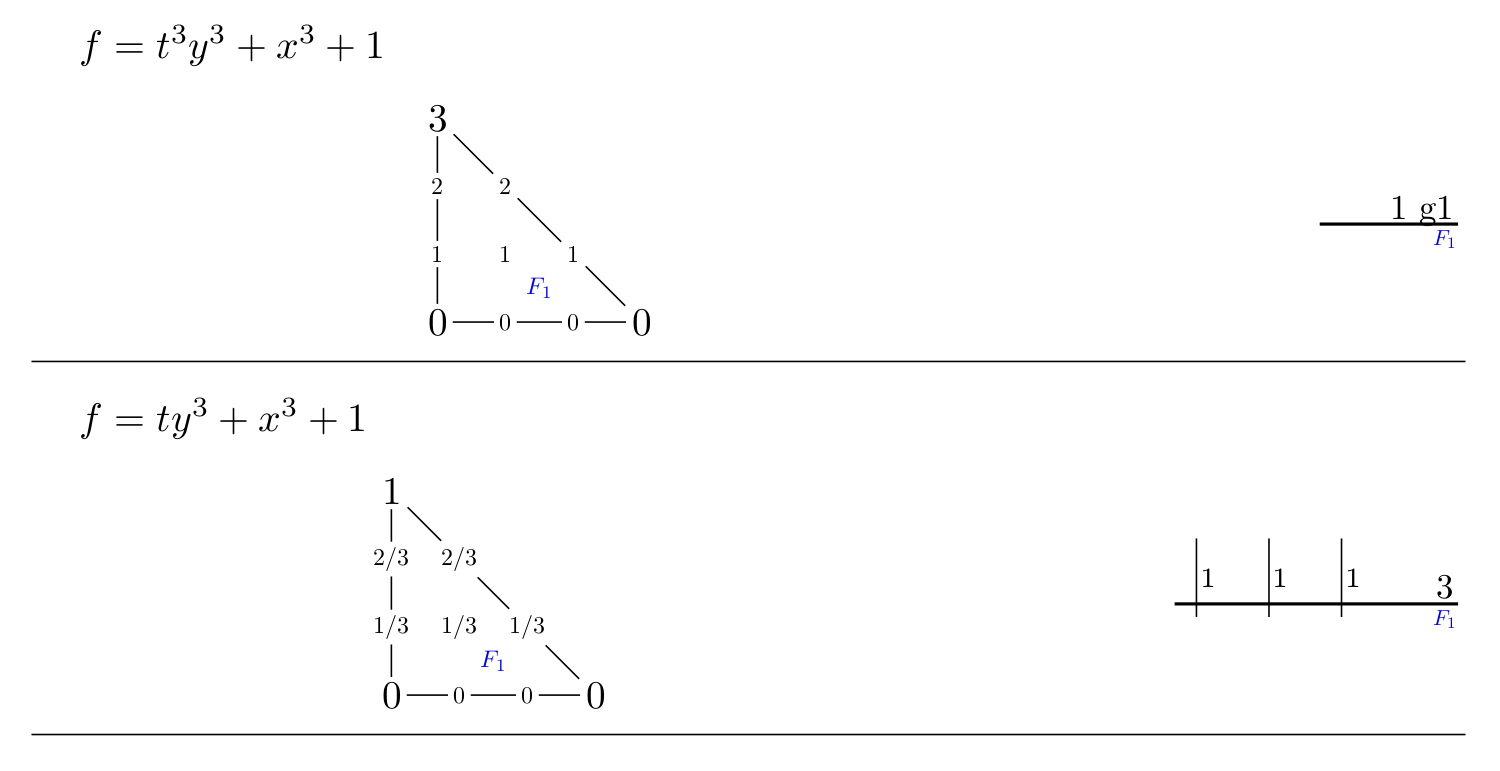
\includegraphics[width=\textwidth]{examples}
\caption[Caption for example]{Partitions of the Newton polygons and the associated graphs of the special fibers corresponding the the equations $f_1 = t^3 y^3 + x^3 + 1$ and $f_2 = t y^3 + x^3 + 1$. (Image created via the software Magma\textsuperscript{1} using scripts by Tim Dokchitser to compute toric models\textsuperscript{2}).
\\
\small\textsuperscript{1} \url{https://magma.maths.usyd.edu.au/magma/}
\\
\small\textsuperscript{2} \url{https://people.maths.bris.ac.uk/~matyd/newton/}}
\end{figure}
\end{example}

\begin{theorem}[Dor18, Thm. 3.13]
Let $f \in K[x^{\pm 1}, y^{\pm 1}]$ be any Laurent polynomial defining a 1-dimensional scheme $C_0 = U_f \subset \Gm{K}^2$. Then $\C_\Delta / R$ is a (proper, flat) model of the toric completion $C = C_0^\Delta$ with respect to the Newton polygon $\Delta = \Delta(f)$. The special fiber $\C_\kappa$ is a union of closed subschemes $\overline{X}_F$ indexed by $\nu$-faces $F$ and chains $X_L \times_\kappa \Gamma_L$ where $\Gamma_L$ is a union of $\P^1_{\kappa}$ intersecting transversally as follows:
\begin{enumerate}
\item for each $\nu$-edge $F$: the scheme $\overline{X}_F$ has multiplicity $\delta_F$ and, via Theorem \ref{baker_refinement} are geometrically connected and have arithmetic genus $ g_F = |\{ P \in F^\circ \cap \Z^2 \mid \nu(P) \in \Z \} | $.
\item for each $\nu$-edge $L$ choose a sequence $\frac{m_i}{d_i} \in \Q$ ($0 \le i \le r+1$) then let $\Gamma_L = \Gamma^1_L \cup \cdots \cup \Gamma^r_L$ with each $\Gamma^i_L$ isomorphic to $\P^1_k$ embedded with multiplicity $\delta_L d_i$ and meeting transversally where we identify $0 \in \Gamma^i_L$ with $\infty \in \Gamma^{i+1}_L$. If $r = 0$ then let $\Gamma_L = \Spec{k}$.
\item The subscheme $X_L \times \{ 0 \} \subset X_L \times \Gamma^1_L$ is identified with $\overline{X}_{F_1} \setminus X_{F_1}$ for the $\nu$-face $F_1$ bordering $L$ and, when $L$ is inner, likewise $X_L \times \{ \infty \} \subset X_L \times \Gamma^r_L$ is identified with $\overline{X}_{F_2} \setminus X_{F_2}$ for the other $\nu$-face $F_2$ bordering $L$. These intersections are transversal and, in fact, as a scheme the intersection is $V(\overline{f_L}^{\delta_L}) \subset X_L \subset \overline{X}_F$. 
\end{enumerate}
Furthermore, the geometrically regular locus of $\C_\Delta$ contains,
\begin{enumerate}
\item the smooth locus of $X_F$, for each $\nu$-face $L$
\item the smooth locus of $X_L \times \Gamma_L$, for each $\nu$-edge $L$
\item the smooth points of $\overline{X}_F \setminus X_F$ corresponding to $L$ when $L \subset \partial F$ is an outer edge with $\delta_L = \delta_F$ and $r = 0$. 
\end{enumerate}
Finally, if $C_0$ is $\Delta_\nu$-regular then $C = C_0^\Delta$ is smooth and thus the unique smooth proper curve birational to $C_0$ and $\C_\Delta / R$ is a regular normal crossings model of $C$. 
\end{theorem}

\section{Relationships Between Toric Notions of Regularity}

We have discussed a number of regularity conditions on curves originating from their compatibility in some sense with a certain set of toric embeddings. The utility of these conditions is the ability to verify them from the equation defining some affine model of the curve in $\Gm{k}^2$. Although these notions are clearly related, we here show that they are, indeed, inequivalent. In this situation, we have a discrete valued field $K$ with valuation ring $R$ and residue field $\kappa$. On the special fiber, we will distinguish between the arithmetic ($\kappa$ non-algebraically closed) and geometric ($\kappa$ arithmetically closed) situations. 

\begin{prop}
Let $C$ be a smooth curve over $K$. Then we have the following implications,
\begin{center}
\begin{tikzcd}
C \text{ is strict } \Delta_\nu \text{-regular} \arrow[Rightarrow, r] \arrow[Rightarrow, d] & C \text{ is nondegenerate } \arrow[Rightarrow, d] 
\\
C \text{ is } \Delta_\nu \text{-regular} \arrow[Rightarrow, r] & C \text{ is weakly nondegenerate}
\end{tikzcd}
\end{center}
Furthermore, no implication is reversible. 
\end{prop}

\begin{proof}
The fact that $\Delta$-nondegeneracy implies weak $\Delta$-nondegeneracy is simply an application of Baker's theorem (recall that this notion was created, by design, as a weaker form of $\Delta$-nondegeneracy, hence the name).  Note that the outer-regular condition introduced in the definition of $\Delta_\nu$-regularity is satisfied when $\overline{X}_F$ is smooth. Thus, $\Delta_\nu$-regularity implies $\Delta_\nu$-regularity since when each of $X_F$ and $X_L$ is smooth then $\overline{X}_F$ is smooth as well via Baker's theorem. 
\par
Strict $\Delta_\nu$-regularity implies that each $X_L$ is smooth thus satisfying the conditions of $\Delta$-nondegeneracy.
Finally, $\Delta_\nu$-regularity implies weak nondegeneracy by the main theorem since if $C_0$ is an affine model in $\Gm{k}^2$ then $C_0^\Delta$ is smooth. Therefore, the affine equation is weakly $\Delta$-nondegenerate with the added condition that $\Delta = \Delta(f)$. Notice that the outer-regularity condition in the definition of a $\Delta_\nu$-regular equation corresponds exactly to the smoothness hypothesis in weak $\Delta$-regularity. So see that strict $\Delta_\nu$-regularity and $\Delta_\nu$-regularity of an equation are not equivalent, let $f \in K[x^{\pm 1}, y^{\pm 1}]$ be a weakly $\Delta$-nondegenerate Laurent polynomial with every term having zero valuation. Then, there is a unique face $F = \Delta(f)$ and for each edge we have $\delta_F = \delta_L = 1$. Then $f$ is $\Delta_\nu$-regular iff it is outer-regular i.e. $U_f^\Delta \subset \Toric_\Delta$ is smooth so $f$ is weakly $\Delta(f)$-nondegenerate. We have seen that weakly $\Delta$-nondegenerate equations need not be $\Delta$-nondegenerate. 
\par
We will give examples showing that nondegenerate curves need not be $\Delta_\nu$-regular.
\end{proof}

\subsection{Genus One Example}

In the arithmetic case, the form of the Galois action on the special fiber comprises an obstruction to having the sort of toric-constructed model described in the previous section. Specifically, the Galois action on the dual graph only permutes ``parallel'' chains of components isomorphic to $\P^1$ therefore each component $\overline{X}_F$ for the faces $F$ must be Galois-invariant, in particular, this includes all positive genus components. Furthermore, note that each component $\overline{X}_F$ is geometrically connected and, by Baker's theorem, smooth when in the $\Delta_\nu$-regular case. Therefore, the special fiber of regular normal-crossings models of $\Delta_\nu$-regular curves cannot have nontrivial orbits of positive genus irreducible components.  
\bigskip\\
To illustrate this phenomenon, we consider the following example. We consider the equicharacteristic case with a section $\kappa \to R$. Choose the ambient scheme,
\[ \P^1_R \times_R \P^1_R = \Proj{R[X_0, X_1]} \times_R \Proj{R[Y_0, Y_1]} \]
and an element $q \in \kappa$. Then we consider the closed subscheme,
\[ X = V((X_0^2 - q X_1^2)(Y_0^2 - q Y_1^2) - \varpi X_0 X_1 Y_0 Y_1) \subset \P^1_R \times_R \P^1_R \] 
where $\varpi \in R$ is the uniformizer. Then $X \to \Spec{R}$ is a regular normal-crossings model of
\[ X_K = V((X_0^2 - q X_1^2)(Y_0^2 - q Y_1^2) - \varpi X_0 X_1 Y_0 Y_1) \subset \P^1_K \times_K \P^1_K \]
This is a smooth curve in $\P^1_K \times_K \P^1_K$ of bidegree $(2, 2)$ and thus genus $g = 1$.
This curve has an affine model,
\[ U = \Spec{k[x, y]/((x^2 - q)(y^2 - q) - \varpi xy)} \subset \A^1_K \times_K \A^1_K \]
Now we consider the special fiber,
\[ X_\kappa = V(X_0^2 - q X_1^2) \cup V(Y_0^2 - q Y_1^2) \subset \P^1_\kappa \times_\kappa \P^1_\kappa \]
The behavior of the special fiber depends of whether $q \in \kappa$ is a square. When $q$ is a non-square, the special fiber has two components $C_1, C_2$ which intersect at two points,
\[ P_{\pm} = (X_0^2 - q X_1^2, Y_0^2 - q Y_1^2, X_0 \mp Y_0) \]
each of order two so $C_i \cdot C_i = -4$ and $[\kappa(C_i) : \kappa] = 2$. Therefore, from the genus formula $g_C = 1$ agreeing with our previous result. Geometrically, each component of the special fiber bifurcates to give four components $C_i$ arranged in a square. Then $C_i \cdot C_i = -2$ since each intersects two other components with a simple intersection so again $g_C = 1$. However, there is a Galois action which flips the square along its diagonal exchanging the opposite pairs of intersection points.
\begin{figure} \label{example_with_P1s}
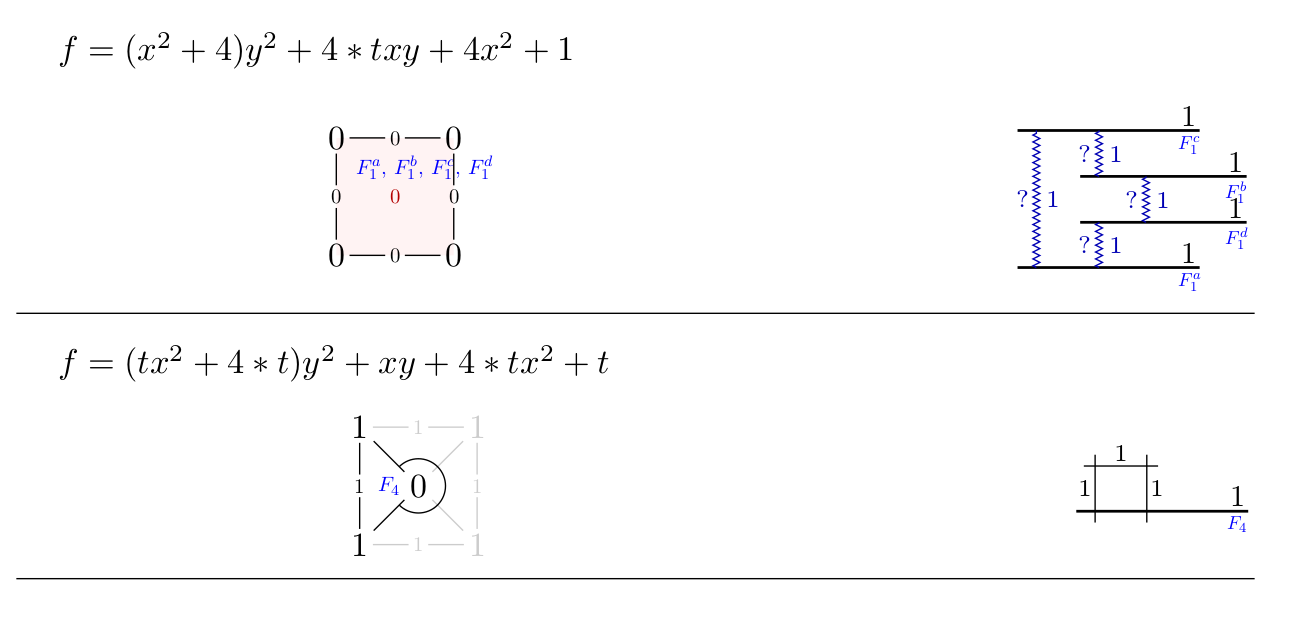
\includegraphics[width=\textwidth]{P1_example}
\caption[Caption for example]{The algorithm applied to $f_1 = (x^2 - 1)(y^2 - 1) - t xy$ and the change of variables $f_2 = uv - t (x^2 - 1)(y^2 - 1)$ chosen to ensure $\Delta_\nu$-regularity. Notice the point of failure of $\Delta_\nu$-regularity in the first case is the singularity of the special fiber which is determined by a single face in this affine presentation. Furthermore, note the topology of the special fiber when it is properly computed. $\Delta_\nu$-regular models are only capable of producing this special fiber in the geometric case i.e. when the components are Galois fixed which occurs when $q \in \kappa$ is a square. However, regardless of $q$, the topology of the special fiber is unchanged with the arithmetic information being encoded in the Galois action instead. (Images created via the software Magma\textsuperscript{1} using scripts by Tim Dokchitser to compute toric models\textsuperscript{2}).
\\
\small\textsuperscript{1} \url{https://magma.maths.usyd.edu.au/magma/}
\\
\small\textsuperscript{2} \url{https://people.maths.bris.ac.uk/~matyd/newton/}}
\end{figure}
\bigskip\\
When $q \in \kappa$ is a non-square, the Galois action on the special fiber does not fix any irreducible component and thus cannot be of the type produced by the previously given toric construction. Therefore, this Galois action may provide an obstruction to finding a $\Delta_\nu$-regular affine equation for $X_K$ despite the fact that we have produced a manifestly $\Delta$-toric affine equation for $X_K$ since $X_K$ is embedded in $\P^1_K \times_K \P^1_K$  via the usual compactification of $f = (x^2 - q)(y^2 - q) - \varpi xy$ with respect to its Newton polygon. To be specific, the r.n.c. model $X$ of the curve $X_K$ cannot be one produced by a $\Delta_\nu$-regular equation. However, the special fiber $X_\kappa$ contains no exceptional curves of the first kind so this is actually a minimal model. In particular, any r.n.c. of $X_K$ may be blown down to $X$. Thus, if $X_K$ had a $\Delta_\nu$-regular equation, this would produce a r.n.c. model $\C_\Delta$ of $X_K$ which can then be blown down to $X$. However, the components of the special fiber of $\C_\Delta$ has fixed points under the $\Gal{\kappa^\sep / \kappa}$-action and thus so does $X_K$. This gives an example of a genus one toric curve (genus one curves are \textit{a priori} toric in any case) which is never-the-less not $\Delta_\nu$-regular.
\bigskip\\
In the case that $q \in \kappa$ is a square, say for definiteness $q = 1$, then the special fiber $X_\kappa$ has the same structure as in the geometric picture except with the Galois action being trivial. It is easy to show that no matter if $q \in \kappa$ is a square or not, the affine equation $f = (x^2 - q)(y^2 - q) - \varpi xy$ is never $\Delta_\nu$-regular because there is a single face which is non-smooth after reduction to $\kappa$. However, in this case this a pathology of the specific choice of affine equation rather than the curve $X_K$. Indeed, performing a change of variables $u_{\pm} = \tfrac{1}{2}(X_0 \pm X_1)$ and $v_{\pm} = \tfrac{1}{2}(Y_0 \pm Y_1)$ which does correspond automorphism of $\P^1_k \times_k \P^1_k$ but not of the torus $\Gm{k}^2$ reflecting the fact that the necessary change of variables must shift the location of the toric divisor in order to be $\Delta_\nu$-regular. Then the homogeneous equation becomes, 
\[ \tilde{f} = 16 u_+ u_{-} v_{+} v_{-} - \varpi (u_{+}^2 - u_{-}^2) (v_{+}^2 - v_{-}^2) \]
Taking the affine patch $D_{+}(u_{-}) \times D_+(v_{-})$ gives an affine model,
\[ U = \Spec{k[u,v]/(16 uv - \varpi (u^2 - 1)(v^2 - 1)} \]
Furthermore, for $p \neq 2$ this equation is $\Delta_\nu$-regular. 


\subsection{Genus Five Example}


In order to extend our argument to higher genus curves, we need to apply Riemann-Roch. However, since this example only works in the arithmetic setting we require a slight modification to the standard statement of Riemann-Roch found in Hartshorne \cite[Thm. IV.1.3]{har}. To ensure there is no confusion, we will provide a proof here.

\begin{theorem}[Riemann-Roch]
Let $X$ be a smooth proper curve over $k$ with $H^0(X, \struct{X}) = K$ and genus $g = \dim_K H^0(X, \omega_X)$. Then for any line bundle $\L$,
\[ \chi(\L) = \dim_k H^0(X, \L) - \dim_k H^0(X, \omega_X \otimes_{\struct{X}} \L^\vee) = \deg{\L} + [ K : k ] (1 - g) \]
Where $\deg{\L}$ is defined in the arithmetic case as follows. Choose a nonzero meromorphic section $s \in H^0(X, \L \otimes_{\struct{X}} \K_X)$ and a local trivialization $\{ (U_i, s_i) \}$ with $s_i \in \L(U_i)$ such that $\struct{U_i} \xrightarrow{s_i} \L|_{U_i}$ is an isomorphism. Then define,
\[ \deg{\L} = \sum_{P \in X} [\kappa(P) : k] \: \ord_{P}(s/s_i) \] 
for some $i$ with $P \in U_i$. 
\end{theorem}

\begin{proof}
First, note that by Serre duality, $H^1(X, \L) \cong H^0(X, \omega_X \otimes_{\struct{X}} \L^\vee)^\vee$ so,
\[ \chi(\L) = \dim_k H^0(X, \L) - \dim_k H^1(X, \L) = \dim_k H^0(X, \L) - \dim_k H^0(X, \omega_X \otimes_{\struct{X}} \L^\vee) \]
Since $X$ is smooth, every line bundle $\L$ is $\struct{X}(D)$ for some divisor $D$. However, since $X$ is smooth, the map $c_1 : \Pic{X} \to \Cl{X}$ is an isomorphism sending,
\[ \L \mapsto \sum_{P \in X} [P] \: \ord_{P}(s_i / s) \]
where the sections $s_i$ and $s$ are as before. Therefore, for a divisor,
\[ D = \sum_{P \in X} n_P \: [P] \]
if we define the degree (including the arithmetic degrees of extensions),
\[ \deg{D} = \sum_{P \in X} [\kappa(P) : k] \: n_P \]
then clearly $\deg{\L} = \deg{c_1(\L)}$. Since $c_1$ is an isomorphism, it suffices to show that,
\[ \chi(\struct{X}(D)) = \deg{D} + 1 - g \]
However, every divisor $D$ can be obtained by a finite sequence of adding or subtracting points $[P]$ from $D = 0$ i.e. from the line bundle $\struct{X}$. Furthermore,
\[ \chi(\struct{X}) = \dim_k H^0(X, \struct{X}) - \dim_k H^1(X, \struct{X}) = [K : k] (1 - g) \]
since, by Serre duality, $\dim_k H^1(X, \struct{X}) = \dim_k H^0(X, \omega_X) = [K : k] g$ because $\dim_K H^0(X, \omega_X) = g$ by definition. Therefore, to proceed by induction, it suffices to show that,
\[ \chi(\L \otimes_{\struct{X}} \struct{X}(\pm P)) = \chi(\L) \pm [\kappa(P) : k] \]
since $\deg{(\L \otimes \struct{X}(\pm P))} = \deg{\L} \pm [\kappa(P) : k]$. Consider the exact sequence,
\begin{center}
\begin{tikzcd}
0 \arrow[r] & \struct{X}(-P) \arrow[r] & \struct{X} \arrow[r] & (\iota_P)_* \kappa(P) \arrow[r] & 0
\end{tikzcd}
\end{center}
where $\kappa(P)$ is the structure sheaf of $P$ as a reduced closed subscheme. Then tensoring by $\L$ we get,
\begin{center}
\begin{tikzcd}
0 \arrow[r] & \L \otimes_{\struct{X}} \struct{X}(-P) \arrow[r] & \L \arrow[r] & (\iota_P)_* \kappa(P) \arrow[r] & 0
\end{tikzcd}
\end{center}
since $\L$ is locally free so $(\iota_P)_* \kappa(P) \otimes_{\struct{X}} \L = (\iota_P)_* \kappa(P)$. Thus,
\[ \chi(\L) = \chi(\L \otimes_{\struct{X}} \struct{X}(-P)) + \chi((\iota_P)_* \kappa(P)) \]
however
\[ \chi(\kappa(P)) = \dim_k H^0(X, (\iota_P)_* \kappa(P)) - \dim_k H^1(X, (\iota_P)_* \kappa(P)) = \dim_k \kappa(P) = [\kappa(P) : k] \]
Therefore,
\[ \chi(\L \otimes_{\struct{X}} \struct{X}(-P)) = \chi(\L) - [\kappa(P) : k] \]
Likewise, replacing $\L$ by $\L \otimes_{\struct{X}} \struct{X}(P)$ we see that,
\[ \chi(\L \otimes_{\struct{X}} \struct{X}(P)) = \chi(\L) + [\kappa(P) : k] \]
proving the theorem. 
\end{proof}

\begin{rmk}
If $s \in H^0(X, \L)$ is a nonzero global section, then we can compute $\deg{\L}$ using the vanishing of $s$ which is effective since $s$ has no poles. Thus, $\deg{\L} \ge 0$. In particular, applying Riemann-Roch to $\omega_X$ we see that $\deg{\omega_X} = \chi(\omega_X) - \chi(\struct{X}) = g - 1 - (1 - g) = 2 g - 2$. Therefore, if $\deg{\L} > 2 g - 2$ then $\deg{(\omega_X \otimes_{\struct{X}} \L^\vee)} = 2 g - 2 - \deg{\L} \le 0$ which implies that $H^0(X, \omega_X \otimes_{\struct{X}} \L^\vee) = 0$ so by Riemann-Roch applied to $\L$ we find,
\[ \dim_k H^0(X, \L) = \deg{\L} + 1 - g \]
\end{rmk}
\noindent\\
Now we consider the following example. Take the field $K = \Fin_p(t)$ with valuation ring $R = \Fin_p[t]_{(t)}$ and residue field $\kappa = \Fin_p$. Given an elliptic curve $C_K$ over $K$ with good reduction $C$ over $\kappa$ so we may take a smooth model $\C$ over $R$. For example, let $q \in \Fin_p^\times$ be a generator, take 
\[ C_K = \Proj{K[X, Y, Z]/(Y^2 Z - X(X^2 - q Z^2)} \] 
we may take the model,
\[ \C = \Proj{R[X, Y, Z]/(Y^2 Z - X(X^2 - q Z^2)} \] 
which is smooth and proper over $R$ for $p \neq 2$. Clearly $\C_K = C_K$ and the special fiber $\C_\kappa$ is the smooth reduction. Now let $P$ be a $\Fin_{p^2}$-point of $C$ which is not a $\Fin_p$-rational points, e.g. take $P = (X^2 - q Z^2, Y)$ which has $\kappa(P) = \Fin_{p^2}$. Recall that $\omega_C = \struct{C}$ since $C$ is an abelian variety and $g = 1$ so if $\deg{\L} > 0$ we know that $\dim_k H^0(C, \L) = \deg{\L}$ be Riemann-Roch. Then consider the line bundle $\L = \struct{C}(P)$ then $\deg{\L} = [\kappa(P) : k]  = 2$. Therefore, we can choose linearly independent sections $s_0, s_1 \in H^0(C, \L)$ where the section $s_0 : \struct{C} \to \L$ is the canonical section defining the closed subscheme $P$ from the inclusion $\L^\vee \to \struct{C}$ of the sheaf of ideals of $P$. Then $s_0$ vanishes exactly on $P$ i.e. the closed subscheme $V(s_0) = P$. Now $\div{(s_1)}$ is an effective divisor of degree $2$ so either $\div{(s_1)} = [P]$ or $\div{(s_1)} = [Q_1] + [Q_2]$ for $\Fin_p$-rational points $Q_1, Q_2$ or $\div{(s_1)} = [Q]$ where $Q \neq P$ is an order-$2$ point. However, if $\div{(s_1)} = [P]$ then $s_1$ must have vanishing order $1$ since it has degree $2$ which implies that $s_0 / s_1 \in H^0(C, \struct{C}^\times)$ contradicting the fact that $s_0$ and $s_1$ are independent in $H^0(C, \L)$ (over $H^0(C, \struct{C}) = \kappa$). The takeaway is that $s_0$ only vanishes at $P$ and $s_1$ does not vanish at $P$. Notice, since we are in equicharacteristic the map $\kappa \to R$, our model is simply a base-change,
\[ \C = C \times_{\Spec{\kappa}} \Spec{R} \]
so we get a line bundle $\L' = \pi_1^* \L$ on $\C$ and, by Kunneth, $H^0(\C, \L') = H^0(C, \L) \otimes_\kappa R$.   
\bigskip\\
We now construct our example as follows. Consider the scheme $\C \times_R \C$ and denote the projection maps, $\pi_i : \C \times_R \C \to \C$. Take the section,
\[ \pi_1^* s_0 \otimes \pi_2^* s_0 - t \: \pi_1^* s_1 \otimes \pi_2^* s_1 \in H^0(\C \times_R \C, \pi_1^* \L' \otimes_{\struct{X}} \pi_2^* \L') \]
on the bundle $\L' \boxtimes \L' := \pi_1^* \L' \otimes_{\struct{X}} \pi_2^* \L'$. We will write this section as $q = s_0 \boxtimes s_0 - t \: s_1 \boxtimes s_1$. Then we take,
\[ X = V(s_0 \boxtimes s_0 - t \: s_1 \boxtimes s_1) \subset \C \times_R \C \]
I claim that $X \to \Spec{R}$ is a regular proper model of,
\[ X_K = V(s_0 \boxtimes s_0 - t \: s_1 \boxtimes s_1) \subset C_K \times_K C_K \]
Here $C_K$ is an elliptic curve over $K$ and I claim that $X_K$ is a smooth projective curve over $K$ of genus $g = 9$. To show this, we compute an affine curve birational to $X_K$. First, we compute the sections $s_0, s_1 \in H^0(X, \struct{C}(P)) \subset K(C)$. Recall that,
\[ H^0(X, \struct{X}(P)) = \{ f \in K(X) \mid \div{(f)} + P \ge 0 \text{ or } f = 0 \} \]
and the canonical section is $s_0 = 1$. Then take $s_1 = \frac{Z}{Y}$ which has, 
\[ \div{(s_1)} = 2 [\infty] - [P] \]
where $[\infty] = [0 : 1 : 0]$ is the point at infinity in the standard $(x, y) = (\frac{X}{Z}, \frac{Y}{Z})$ coordinates\footnote{For $P = (X^2 - g Z^2, Y)$ the intuitive choice $s_1 = (\frac{X^2}{Z^2} - q)^{-1}$ will not give a section of $\struct{C}(P)$ because its vanishing order is too large, in fact, $\ord_{P}{(\frac{X^2}{Z^2} - q)} = 2$. To see this, consider the affine patch $D_{+}(Z)$ with coordinates $(x, y) = (\frac{X}{Z}, \frac{Y}{Z})$ and the section $(x^2 - q) \in A_{P}$ where $A = \kappa[x, y]/(y^2 - x(x^2 - q))$. Let $\m = P A_P$ then clearly $(x^2 - q) \in \m$ but also $(x^2 - q) \in \m^2$ because $x^{-1} y^2 = (x^2 - q) \in \m^2$ since $y \in \m$ and $x \notin P$.}. To compute $\div{(s_1)}$, note that $\ord_{P}(y) = 1$ because $y \in (x^2 - q, y)$ but $y \notin (x^2 - q, y)^2$, furthermore, in $D_+(Y)$ and local coordinates $(x,z) = (\frac{X}{Y}, \frac{Z}{Y})$ then $s_1 = z$ and $\ord_{\infty}(z) = 2$ because $z \in (x, z)$ and $z \in (x, z)^2$ since $z = x(x^2 - q z^2) \in (x, z)^2$. 
\bigskip\\
We choose the affine patch, $U_K \times_K U_K \subset C_K \times_K C_K$ which is defined by,
\[ U_K = C_K \cap D(Z) = \Spec{K[x,y]/(y^2 - x(x^2 - q))} \]
Since $\div{(\frac{Y}{Z})} = [P] - 2 [\infty]$, applying the exact sequence,
\begin{center}
\begin{tikzcd}
\lbrack \infty \rbrack \cdot \Z \arrow[r] & \Cl{C_K} \arrow[r] &  \Cl{U_K} \arrow[r] & 0
\end{tikzcd}
\end{center}
we see that $[P] \in \Cl{U}$ is principal $[P] = \div{(\frac{Z}{Y})}|_U$. Therefore, $\struct{C_K}(P) \cong \struct{C_K}$ via the isomorphism, $1 \mapsto \frac{Y}{Z}$ meaning that $s_0 \mapsto \frac{Y}{Z}$ and $s_1 \mapsto 1$ in $\struct{C_K}$. Therefore, the affine open,
\[ V_K = V(s_0 \boxtimes s_0 - t \: s_1 \boxtimes s_1) \subset U_K \times_K U_K \]
is explicitly,
\[ V_K = \Spec{K[x_1, y_1, x_2, y_2]/(y_1^2 - x_1(x_1^2 - q), y_2^2 - x_2(x_2^2 - q), y_1 y_2 - t)} \]
In the software sage\footnote{\url{http://www.sagemath.org/}}, we can compute the genus $g = 5$ from this affine presentation \footnote{In fact, asking sage to compute the genus of the above affine curve produces $g = 10$. This reflects that sage computes the genus \textit{over the field of definition} where as we take the base field here to be $k = H^0(X, \struct{X})$ and define $g = \dim_k H^0(X, \Omega^1_X)$. In our example here, since $P$ is an order two point, $H^0(X, \struct{X}) = \Fin_{p^2}$ and thus, the correct genus is computed as,
\[ g(X) = \dim_\kappa H^0(X, \Omega^1_X) / \dim_\kappa H^0(X, \struct{X}) = 10/2 = 5 \]}.
Now consider the special fiber $X_\kappa = V(s_0 \boxtimes s_0) \subset C \times_k C$ given by the base change under the map $R \to R/(t) = \kappa$ sending $t \mapsto 0$. Therefore, the irreducible components $C_1, C_2$ are each isomorphic to $C \times_{\Fin_p} \Fin_{p^2}$ and as effective Cartier divisors $X_\kappa = C_1 + C_2$ with multiplicity one since the special fiber is reduced. The intersection number between these components is $C_1 \cdot C_2 = 4$ because these components intersect at two points $P_{\pm} = (X_0^2 - q Z_0^2, Y_0, X_1^2 - q Z_1^2, Y_1, X_0 \mp X_1)$ each a point of degree $2$. Therefore, using $C_i \cdot (C_1 + C_2) = 0$ we find that $C_i \cdot C_i = -4$. Therefore, applying the genus formula,
\[ g_C = 1 + \sum_{i = 1}^n m_i \left( [\kappa(C_i) : \kappa] (g_{C_i} - 1) - \frac{1}{2} (C_i \cdot C_i) \right) \]
we get $g_C = 1 + 4 = 5$ since $g_{C_i} = 1$ and $m_i = 1$ because each component is a reduced elliptic curve. 
\bigskip\\
Geometrically, each component bifurcates to give a square with each side a reduced elliptic curve divisor isomorphic to $C$. The Galois group acts on this square by reflection across the diagonals. Since $X$ does not contain any exceptional curves of the first kind, it is the minimal model of $V$ (and in fact the minimal regular normal crossings model since $X_\kappa$ happens to be a normal crossings divisor). Therefore, any proper regular normal crossings model of $V$ must be a blowup of $X$ and, in particular, its special fiber must contain two pairs of Galois conjugate elliptic curves. Therefore, no $\Delta_\nu$-regular affine equation for $V$ can exist since such an equation would define a proper regular normal crossings model of $V$ with trivial Galois action on positive genus components. 